\documentclass{standalone}
\usepackage{pgfplots}
\pgfplotsset{compat=1.18}
\usepgfplotslibrary{colorbrewer}
\pgfplotsset{cycle list/Set1-6}

\begin{document}

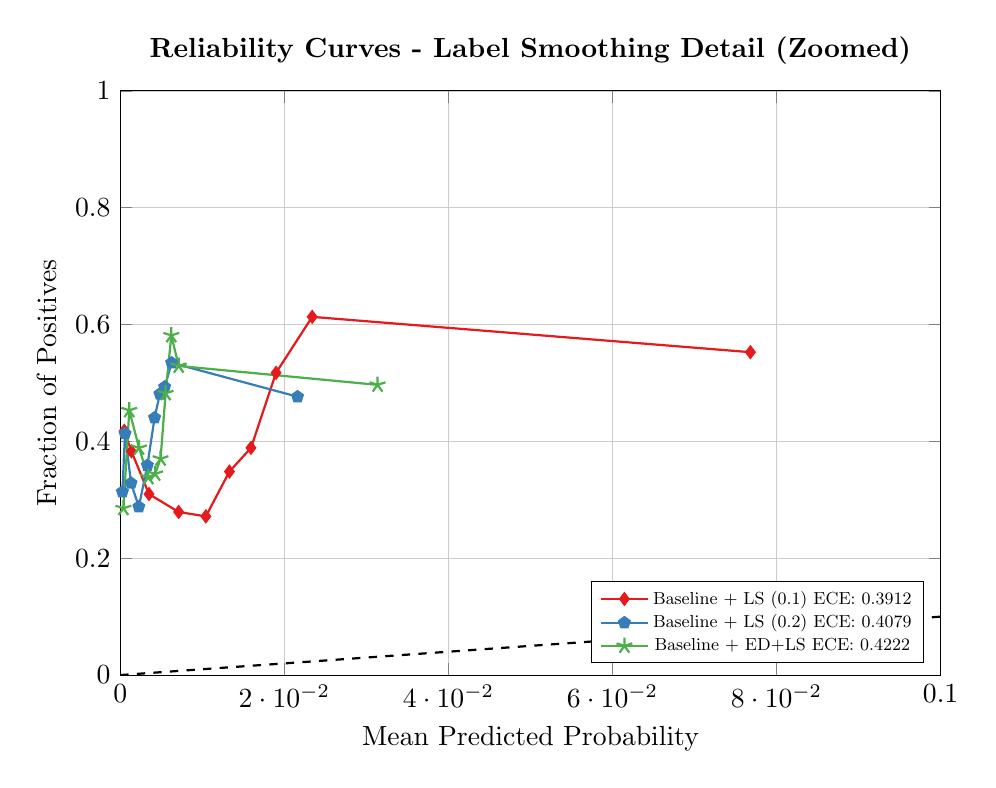
\begin{tikzpicture}
\begin{axis}[
    title={\textbf{Reliability Curves - Label Smoothing Detail (Zoomed)}},
    xlabel={Mean Predicted Probability},
    ylabel={Fraction of Positives},
    xmin=0, xmax=0.1, % Expanded X-axis focus
    ymin=0, ymax=1,
    xtick={0, 0.02, 0.04, 0.06, 0.08, 0.1},
    ytick={0, 0.2, 0.4, 0.6, 0.8, 1.0},
    legend pos=north east,
    legend style={nodes={scale=0.7, transform shape}, font=\small},
    grid=both,
    grid style={line width=.1pt, draw=gray!20},
    major grid style={line width=.2pt, draw=gray!40},
    width=12cm,
    height=9cm,
    cycle list name=Set1-6,
    % Shift legend to avoid overlapping data
    legend style={at={(0.98,0.02)}, anchor=south east}
]

% Perfectly Calibrated Line (Visible in the zoom)
\addplot [color=black, dashed, line width=0.8pt, forget plot]
    coordinates {(0,0)(0.1,0.1)};

% Model 4: Baseline + Label Smoothing (0.1)
\addplot+[mark=diamond*, thick] coordinates {
    (0.0004922,  0.41817294) (0.00136182, 0.38309309) (0.00350409, 0.30979721) 
    (0.00711733, 0.27925727) (0.01043486, 0.27168336) (0.01330828, 0.34839971) 
    (0.01593354, 0.38895676) (0.01899207, 0.51746885) (0.02339561, 0.61324212) 
    (0.07681628, 0.55276014)
};
\addlegendentry{Baseline + LS (0.1) ECE: 0.3912}

% Model 5: Baseline + Label Smoothing (0.2)
\addplot+[mark=pentagon*, thick] coordinates {
    (0.00026047, 0.3136297)  (0.00058063, 0.41338871) (0.0013168,  0.32860982) 
    (0.00226386, 0.28805277) (0.00330721, 0.35890545) (0.00418406, 0.44050818) 
    (0.00483144, 0.48130955) (0.00541067, 0.49328121) (0.00626516, 0.53457122) 
    (0.02161047, 0.47655105)
};
\addlegendentry{Baseline + LS (0.2) ECE: 0.4079}

% Model 6: Baseline + Edge Dropout (0.2) + Label Smoothing (0.1)
\addplot+[mark=star, thick, mark size=3pt] coordinates {
    (0.0003858,  0.28553981) (0.00109858, 0.4532128)  (0.0022893,  0.38895676) 
    (0.00342556, 0.3383826)  (0.00425036, 0.34449059) (0.00491393, 0.37038847) 
    (0.00552733, 0.48228683) (0.00622427, 0.58148058) (0.00712705, 0.52919619) 
    (0.03136405, 0.49682462)
};
\addlegendentry{Baseline + ED+LS ECE: 0.4222}

\end{axis}
\end{tikzpicture}
\end{document}